\documentclass[letterpaper]{article}
\title{EE 511 Machine Learning, Winter 2018: Homework 2}
\date{Due: Wednesday, January $31^{st}$, beginning of class}
\usepackage{hyperref}

\usepackage[margin=1in]{geometry}

\usepackage{amsmath,amsfonts}
\usepackage{url}
\usepackage{graphicx}
\usepackage{color}
\usepackage{enumerate}
\usepackage{bbm}
\providecommand{\m}[1]{\mathbf{#1}}
\providecommand{\norm}[1]{\left\|#1\right\|}
\providecommand{\sign}[1]{\text{sign}\left(#1\right)}
\DeclareMathOperator*{\argmin}{arg\,min}
\providecommand{\w}{\m{w}}
\providecommand{\what}{\hat{w}}

\begin{document}

\maketitle

\section{Fitting an SVM classifier by hand [50 Points]}

(Source: Murphy text, Exercise 14.1) Consider a dataset with 2 points in 1d:

\begin{center}
$(x_1 = 0, y_1 = -1)$ and $(x_2 = \sqrt{2}, y_2 = 1)$.
\end{center}

Consider mapping each point to 3d using the feature vector
$\phi(x) = [1,\sqrt{2}x, x^2]^T$ 
(This is equivalent to using a second order polynomial kernel).
The max margin classifier has the form

\begin{equation}
\what,\hat{w_0} = \argmin ||w||^2 \quad s.t.
\label{eq:objective}
\end{equation}
\vspace{-1cm}

\begin{equation}
y_1(w^T \phi(x_1) + w_0) \geq 1
\label{eq:condit1}
\end{equation}
\vspace{-1cm}

\begin{equation}
y_2(w^T \phi(x_2) + w_0) \geq 1
\label{eq:condit2}
\end{equation}

\begin{enumerate} \item (10 Points) Write down a vector that is
parallel to the optimal vector $\what$. Hint: Recall that $\what$ is perpendicular to the decision boundary between
the two points in the 3d feature space. \\

\item (10 Points) What is the value of the margin that is achieved by
this $\what$? Hint: Recall that the margin is the distance from each support
vector to the decision boundary. Hint 2: Think about the geometry of the points
in feature space, and the vector between them. \\

\item (10 Points) Solve for $\what$, using the fact the margin is equal
to $1/||\what||$. \\

\item (10 Points) Solve for $\hat{w_0}$ using your value for $\what$
and Equations \ref{eq:objective} to \ref{eq:condit2}. Hint: The points will be
on the decision boundary, so the inequalities will be tight. A ``tight
inequality'' is an inequality that is as strict as possible. For this problem,
this means that plugging in these points will push the left-hand side of
Equations \ref{eq:condit1} and \ref{eq:condit2} as close to $1$ as possible. \\

\item (10 Points) Write down the form of the discriminant function
$f(x) = \hat{w_0} + \what^T\phi(x)$ as an explicit function of $x$. Plot the 2
points in the dataset, along with $f(x)$ in a 2d plot. You may generate this
plot by hand, or using a computational tool like Python. \\ 

\end{enumerate}

\section{Perceptrons [50 points]}
Recall that a perceptron learns a linear classifier with weight vector $w$. It predicts 
$$
y^{(i)} = \text{sign}(w^Tx^{(i)})
$$
(assuming here that $y^{(i)} \in \{+1,-1\}$. Also, note that we are \emph{not} using a bias
weight $w_0$, for simplicity). When the perceptron makes a mistake, it updates the weights
using the formula
$$
w = w + y^{(i)} x^{(i)} 
$$

Imagine that we have $x^{(i)} \in \mathbb{R}^2$, and we encounter the following data points
\begin{center}
\begin{tabular}{c|c|c}
    $x_1$ & $x_2$ & $y$ \\
    \hline
    1 & 1 & 1 \\
    2 & -1 & -1 \\
    -3 & -1 & -1 \\
    -3 & 1 & 1 \\
\end{tabular}
\end{center}

\begin{enumerate}
%\newpage
\item (25 points)
    Starting with $w = [0\quad0]^T$, use the perceptron algorithm to learn on the data points
    in the order from top to bottom. Show the perceptron's linear decision boundary after
    observing each data point in the graphs below. Be sure to show which side is classifed
    as positive.

		\begin{figure}[h]
			\begin{center}
				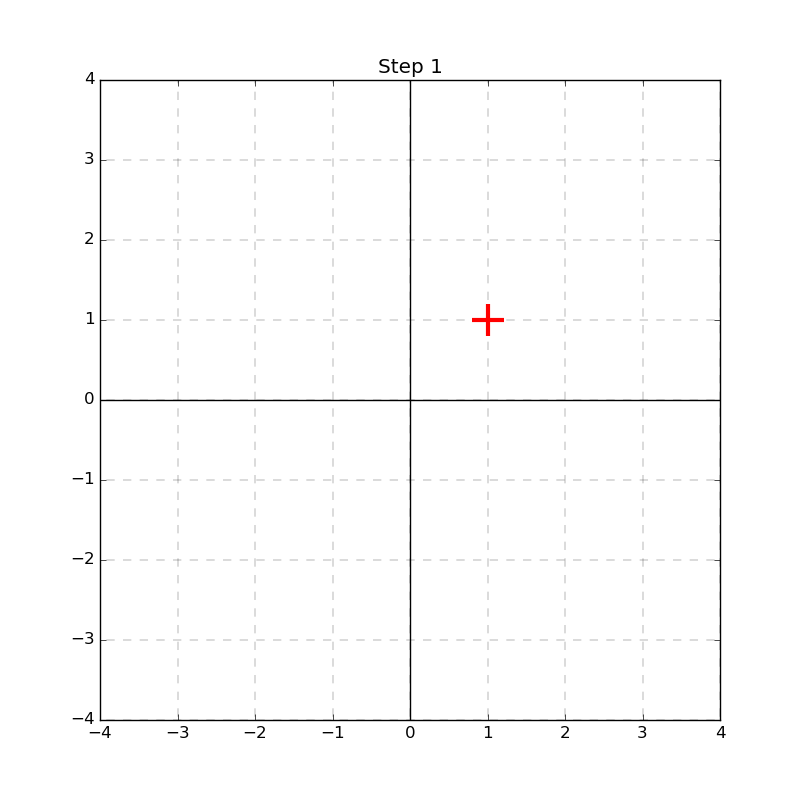
\includegraphics[width=0.4\textwidth]{1.png}
				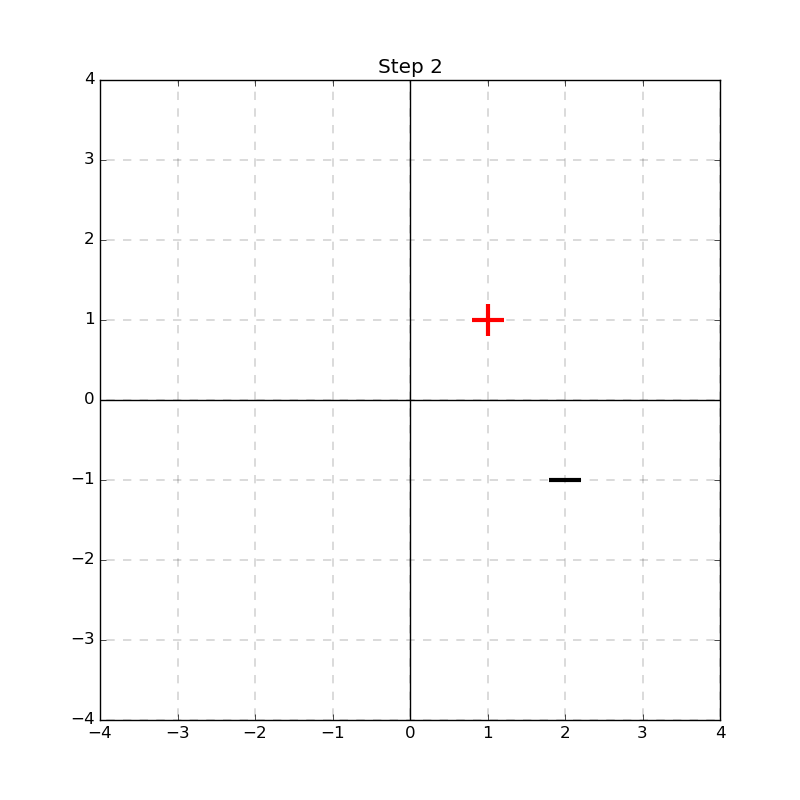
\includegraphics[width=0.4\textwidth]{2.png}
				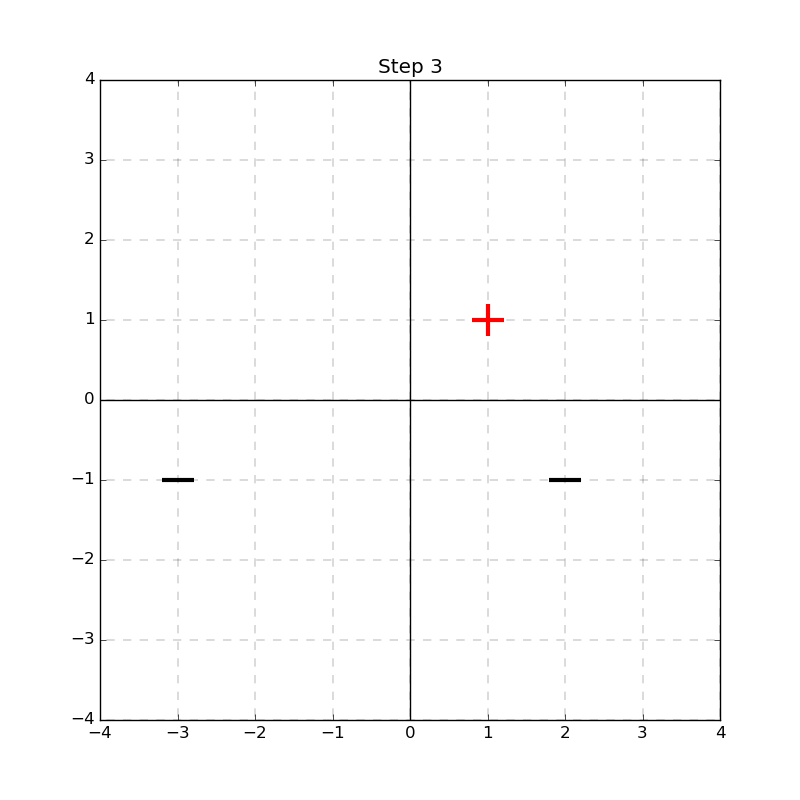
\includegraphics[width=0.4\textwidth]{3.png}
				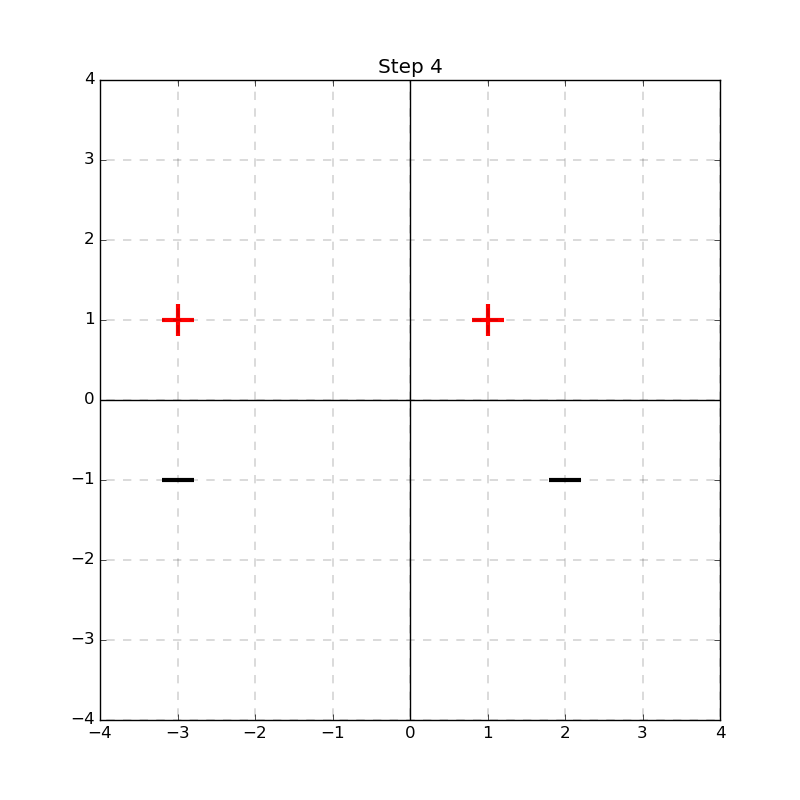
\includegraphics[width=0.4\textwidth]{4.png}
			\end{center}
		\end{figure}


%\newpage
\item (10 points) 
    Does our learned perceptron maximize the margin between the training data and the decision
    boundary? If not, draw the maximum-margin decision boundary on the graph below.

\begin{center}
    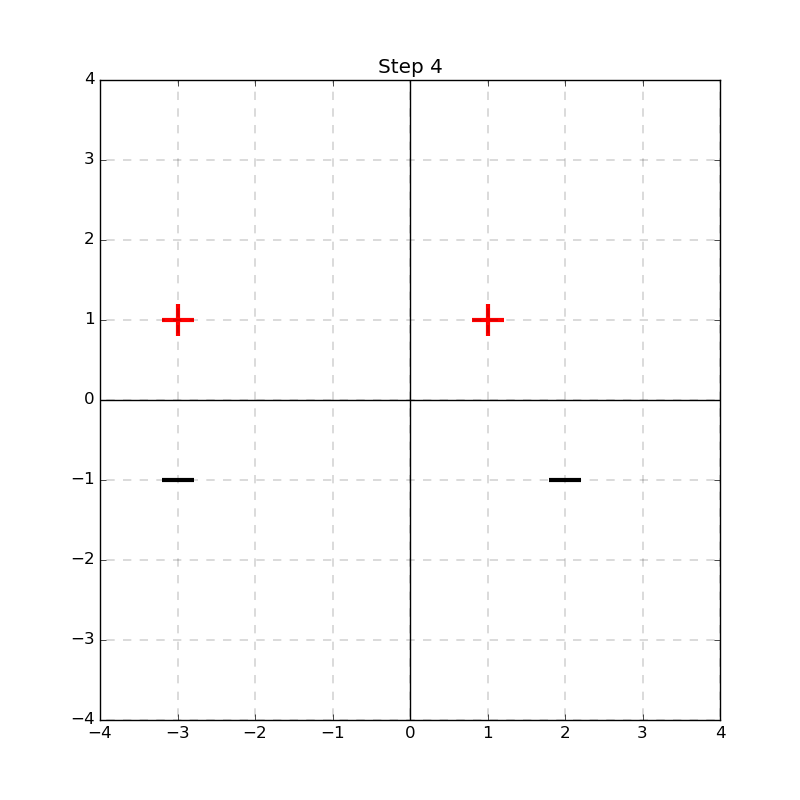
\includegraphics[width=0.4\textwidth]{4.png}
\end{center}
\vspace{1in}
\item (15 points)
    Assume that we continue to collect data and train the perceptron. If all data we see (including
    the points we just trained on) are linearly separable separable with margin $\gamma = 0.5$ and
    have maximum norm $||x^{(i)}|| \leq 5$, what is the maximum number of mistakes we can make on
    future data?
\vspace{2in}
\end{enumerate}

\section{Logistic Regression [100 points]}
In this assignment, you will be predicting income from census data using
logistic regression. Specifically, you will predict the probability that a
person earns more than \$50k per year. For more details about the dataset,
please visit \url{http://www.cs.toronto.edu/~delve/data/adult/adultDetail.html}.

Please download the code.zip file. In the code fold, you will be modifying the
file \textbf{sgd.py}. Tests for your program are in \textbf{test.py}. 
To test your implementation, run: \texttt{python test.py}.
\begin{itemize}
	\item (10 points) 
		\textbf{Logistic Function}:
		To perform logistic regression you have to be able to calculate the logistic
		function.  Fill in the \texttt{logistic} function.

	\item (5 points)
		\textbf{Dot Prodct:}
		The model you are training is just a bunch of numerical weights. To run your
		model on a data points you will need to take the dot product of your weights
		and the features for that data point and run the result through your
		logistic function.  First fill in the \texttt{dot} function to take the dot
		product of two vectors 

	\item (5 points)
		\textbf{Prediction:}
		Now that you can calculate the dot product, predicting new data points
		should be easy! Fill in the \texttt{predict} function to run your model on a
		new data point. Take a look at \texttt{test.py} to see what the format for
		data points is.

		Prediction should be straightforward, to predict new points you simply
		multiply your model's weights by the corresponding features, sum up the
		result, and pass it through the logistic function. This should be easy with
		your dot product and logistic functions.

	\item (10 points) Once you start training your model you are going to want to
		know how well you are doing. Modify the \texttt{accuracy} function to
		calculate your accuracy on a dataset given a list of data points and the
		associated predictions.

	\item (20 points) 
		\textbf{Train Your Model:}
		Fill in the \texttt{train} and \texttt{update} functions to train your
		model! You should use logistic regression with L2 regularization where
		\texttt{rate} is the learning rate and \texttt{lam} is the regularization
		parameter.

		The training should run for some number of epochs performing stochastic
		gradient descent.
		
		This means you will randomly select a point from the dataset and run the
		model on that data point. Then you will calculate the error for that point
		and adjust your model weights based on the gradient of that error. An epoch
		refers to a full pass over the dataset. In practice it is easier (and more
		statistically valid) to sample randomly with replacement. Thus an epoch just
		means examining N data points where N is the number of points in your
		training data.
		
		This is different than batch gradient descent where you look at all of the
		data points before updating. SGD converges faster but can also be less
		stable because you have a noisy estimate of the gradient instead of the true
		gradient. In practice it is often much better to use SGD than full batch
		gradient descent.

		When you see a new data point, you prediction will be:
		\begin{verbatim}
Prediction = P(income > 50k | W, x) = logistic(W��x)
		\end{verbatim}

		Your loss function will be:
		\begin{verbatim}
			Loss = (Prediction - Truth)^2 + Lambda * || W ||
		\end{verbatim}
		By minimizing this loss, the model learns to make correct predictions and
		also use small weights to avoid overfitting.

		To adjust the model you have to calculate the gradient of the loss at a
		given point. The gradient will come from two sources, the error and the
		regularization.

		While this minimizing this loss looks different than maximizing the
		conditional log likelihood, the gradient is actually the same, just with
		opposite sign. Thus you can either descend the gradient of this loss
		function or ascend the gradient of the conditional log likelihood and you
		will be performing the same updates. If you want, you can derive why this is
		the case by taking the partial derivative of the above loss function with
		respect to a single weight in the model. Use the update rule from class to
		adjust the model, but remember, since we are doing SGD you only look at one
		point before updating the model:
		\begin{eqnarray*}
			w_i^{(t+1)}\leftarrow w_i^{(t)} + \eta\left(
				-\lambda w_i^{(t)} +
				\sum_j x_i^j \left[
					y^j - \hat{P}(Y^j=1|\textbf{x}^j, \textbf{w})
				\right]
			\right)
		\end{eqnarray*}

		When you run python \texttt{test.py} it will tell you your current accuracy
		on the training and validation set. By default these are the same dataset!
		To get a more accurate evaluation you can modify \texttt{data.py} to use
		different training and validation sets by splitting your data.

	\item (20 points)
		\textbf{Extract Better Features:}
		Take a look at the feature extracting code in \texttt{extract\_features},
		and at the raw data in adult.data. Right now your model is only considering
		age, education, and one possible marital status.

		Good feature extraction is often the key to making good machine learning
		models. Add more feature extraction rules to help improve your model's
		performance. This is very open ended, be creative and find features that
		work well with your model.


	\item (30 points)
		\textbf{Tune Your Submission:}
		Tune your \texttt{submission} function to train your final model. You should
		change your feature extraction and training code to produce the best model
		you can.  Try different learning rates and regularization parameters, how do
		they compare? Often it is good to start with a high learning rate and
		decrease it over time, feel free to add this to your training code.

		Your final model will be trained on the full training data and run on test
		data that you don't have access to. Your grade for this section will be
		based on your performance relative to an untuned baseline and to the other
		other students in class. Good luck!

	\item Only submit your modified \texttt{sgd.py} file.

\end{itemize}

\end{document}
